\documentclass[a4paper,12pt,bibliography=totoc, listof=totoc,titlepage]{scrreprt}
\usepackage[ngerman]{babel}
\usepackage[utf8]{inputenc}
\usepackage[left=3cm,right=2.5cm,top=2.5cm,bottom=2.5cm]{geometry}
\usepackage[onehalfspacing]{setspace}
\renewcommand{\arraystretch}{1.5}
\usepackage{graphicx}
\usepackage{color}
\usepackage[dvipsnames,usenames,dvipsnames,table,xcdraw]{xcolor}
\usepackage[toc,page]{appendix}
\usepackage[printonlyused]{acronym}
%\usepackage[scaled]{berasans}
%\renewcommand*\familydefault{\sfdefault}  %% Only if the base font of the document is to be sans serif
%\usepackage[T1]{fontenc}

% Absatz-Einstellungen
\setlength{\parindent}{15pt} % Einrücken
\setlength{\parskip}{6pt}  % Horizontaler Abstand

\usepackage{subcaption}
\usepackage{graphicx} % omit 'demo' for real document
  
\usepackage[hyphens]{url}
\usepackage[hidelinks]{hyperref}
\setlength {\marginparwidth }{2cm}
\usepackage{todonotes}
\usepackage{amsmath}
\usepackage{cancel}

% Kommentare mit \begin{comment}
\usepackage{verbatim}

\usepackage{multirow}

\newcommand*\justify{%
  \fontdimen2\font=0.4em% interword space
  \fontdimen3\font=0.2em% interword stretch
  \fontdimen4\font=0.1em% interword shrink
  \fontdimen7\font=0.1em% extra space
  \hyphenchar\font=`\-% allowing hyphenation
}

\newcommand{\code}[1]{\texttt{\justify{#1}}}
%\usepackage{tocloft}

%Boxfehler
\hbadness=1000000

% Hurenkinder und Schusterjungen verhindern
\clubpenalties 4 10000 10000 1000 1000
\widowpenalties 4 10000 10000 1000 1000
\displaywidowpenalty=10000

% Listings
\usepackage{listings}
\lstset{
   breaklines=true,
   captionpos=t,
   basicstyle=\scriptsize\ttfamily,
   keywordstyle=\bfseries\ttfamily\color{orange},
   stringstyle=\color{green}\ttfamily,
   commentstyle=\color{gray}\ttfamily,
   emph={square}, 
   emphstyle=\color{blue}\texttt,
   emph={[2]root,base},
   emphstyle={[2]\color{yac}\texttt},
   showstringspaces=false,
   flexiblecolumns=false,
   tabsize=2,
   numbers=left,
   numberstyle=\tiny,
   numberblanklines=false,
   stepnumber=1,
   numbersep=10pt,
   xleftmargin=15pt
 }

% Zitierstil
%\usepackage[style=authoryear,citestyle=authoryear,natbib=true]{biblatex}
%\bibliography{Thesis.bib}
\usepackage[round]{natbib}
\bibliographystyle{hcu}

\begin{document}
\pagenumbering{Roman}
\begin{titlepage}
    \begin{center}
        \renewcommand{\arraystretch}{0.7}
        \begin{tabular}{lr}
            \begin{tabular}{l}
                
\includegraphics[width=0.35\textwidth]{img/hculogo_grau.png}
            \end{tabular} \hspace{1.2cm} &
            \begin{tabular}{r}
                Universität für           \\Baukunst und Metropolenentwicklung\\
                Henning-Voscherau-Platz 1 \\
                20457 Hamburg             \\
            \end{tabular}
        \end{tabular}\\\vspace{5cm}
        \doublespacing
        {\huge\bfseries Aufbau eines photogrammetrischen Messsystems unter Verwendung von Rasberry-Pi-Kameras als Low-Cost-Sensoren }\vspace{0.5cm}\\

        {\large\bfseries Geodäsie und Geoinformatik\\Masterthesis\\Sommersemester 2024}\vspace{2cm}\\
        {\large Florian Timm}

        % hspace und vspace bedeutet horizontaler bzw. vertikaler Abstand
        \vspace{7cm}
        Abgabedatum: 01. August 2024
    \end{center}
    \setcounter{page}{0} % Seitenzahl wird auf 0 gesetzt 
\end{titlepage}


\vspace{2cm}
\noindent\textbf{\large Verfasser}\\
Florian Timm\\
Matrikelnummer: 6028121\\
Gaiserstraße 2, 21073 Hamburg\\
\\
E-Mail: florian.timm@hcu-hamburg.de\\
\vspace{3cm}\\
\noindent\textbf{\large Erstprüfer}\\
Prof. Dr.-Ing. Thomas Kersten\\
HafenCity Universität Hamburg\\
Überseeallee 16, 20457 Hamburg\\
\\
E-Mail: thomas.kersten@hcu-hamburg.de\\
\vspace{3cm}\\
\textbf{\large Zweitprüfer}\\
Dipl.-Ing. Kay Zobel\\
HafenCity Universität Hamburg\\
Überseeallee 16, 20457 Hamburg\\
\\
E-Mail: kay.zobel@hcu-hamburg.de\\
\newpage
\noindent\textbf{\large Kurzzusammenfassung}\\
Die Photogrammetrie bietet die Möglichkeit, mit relativ einfacher Technik 3D-Modelle zu erstellen. Die Aufnahme der Bilder ist jedoch sehr zeitaufwendig und daher für die Erfassung vieler Objekte, z.B. bei der Digitalisierung von Museumsobjekten, nicht praktikabel. Systeme mit mehreren fest installierten Kameras setzen in der Regel auf hochwertige Kameras, die jedoch die Hardwarekosten stark in die Höhe treiben.

In dieser Arbeit soll der Lösungsansatz untersucht werden, mehrere kostengünstige Kameras, die fest auf einem Rahmen montiert sind, zu verwenden. Mit Kameras für den Raspberry Pi soll ein photogrammetrisches Messsystem für kleine Objekte aufgebaut werden. Dazu soll eine Schnittstelle zur Synchronisation der Kameras programmiert und eine Möglichkeit zur Kalibrierung der Kameras entwickelt werden. Das Endergebnis soll es im Idealfall auch einem photogrammetrischen Laien ermöglichen, schnell und ohne lange Einarbeitungszeit 3D-Modelle in akzeptabler Auflösung und Qualität zu erzeugen.
\vspace{2cm}\\
\noindent\textbf{\large Abstract}\\
Photogrammetry offers the possibility of creating 3D models with relatively simple technology. However, capturing the images is very time consuming and therefore not practical for many objects, such as museum digitisation. Systems using multiple fixed cameras usually rely on high quality cameras, which significantly increases hardware costs.

This paper explores the solution of using multiple low-cost cameras mounted on a frame. Cameras for the Raspberry Pi are used to build a photogrammetric measurement system for small objects. This involves programming an interface to synchronise the cameras and developing a way to calibrate the cameras. The end result should ideally enable even a photogrammetric layman to produce 3D models of acceptable resolution and quality quickly and without a long training period.

% Mehrere gleichzeitig zitieren
\providecommand{\citeTwo}[4]{\citep[{\citealp[#1]{#2};}][#3]{#4}}
\providecommand{\citeThree}[6]{\citep[{\citealp[#1]{#2}; \citealp[#3]{#4};}][#5]{#6}}
\providecommand{\citeFour}[8]{\citep[{\citealp[#1]{#2}; \citealp[#3]{#4}; \citealp[#5]{#6};}][#7]{#8}}

\newpage

\tableofcontents
\newpage

\pagenumbering{arabic}
\setcounter{page}{1}

\chapter{Konzept}
In Museen besteht vielfach der Wunsch, ihre Exponate zu digitalisieren. Entsprechende Handreichungen des Deutschen Museumsbundes legen auch die Digitalisierung als 3D-Modelle nahe, verweisen aber auf Aufwand und Format-Probleme \citep[S. 43]{handreichung_digital}.
Auch bei Ausgrabungen aber auch in anderen Bereichen besteht der Bedarf dreidimensionale Modelle einfach und kostengünstig zu erfassen.

Diese Möglichkeit soll das im Rahmen dieser Arbeit entwickelte Kamerasystem bieten. Es soll mittels Photogrammetrie ermöglichen, mit geringen personellen Aufwand kleine Objekte bis etwa 40~cm Durchmesser zu erfassen. Die Bedienung soll dabei laiensicher und mit nur kurzer Einarbeitungszeit möglich sein, dass System also die meisten Schritte selbstständig durchführen. Auch der Nachbau soll mit etwas handwerklichen Geschick möglich sein. Um Lizenzkosten zu sparen, soll die Möglichkeit auf OpenSource-Software zu setzen geprüft werden.

Neben der eigentlichen Entwicklung eines funktionsfähigen Systemes soll abschließend die Anzahl der Kameras und die Nutzung eines Drehtellers evaluiert werden, um hiermit gegebenenfalls die Hardwarekosten zu senken oder die Auflösung und Genauigkeit zu steigern.

\chapter{Photogrammmetrischer Hintergrund}
\label{c:photogrammmetrie}
Das Erzeugen des 3D-Modelles basiert auf der Verknüpfung von Bildern aus verschiedenen Positionen über identische Punkte. Hieraus können dann die Orientierung der Kameras zueinander und die Koordinaten der Punkte in einem lokalen Koordinatensystem ohne bekannten Maßstab berechnet werden. Durch die Nutzung von bekannten Größen beispielsweise durch Maßstäbe kann dieses System transformiert werden.

Dieses Kapitel beschreibt die hierfür notwendigen Bedingungen und die Grundlagen der Rekonstruktion des Objektes als 3D-Modell.

\begin{figure}
    \centering
    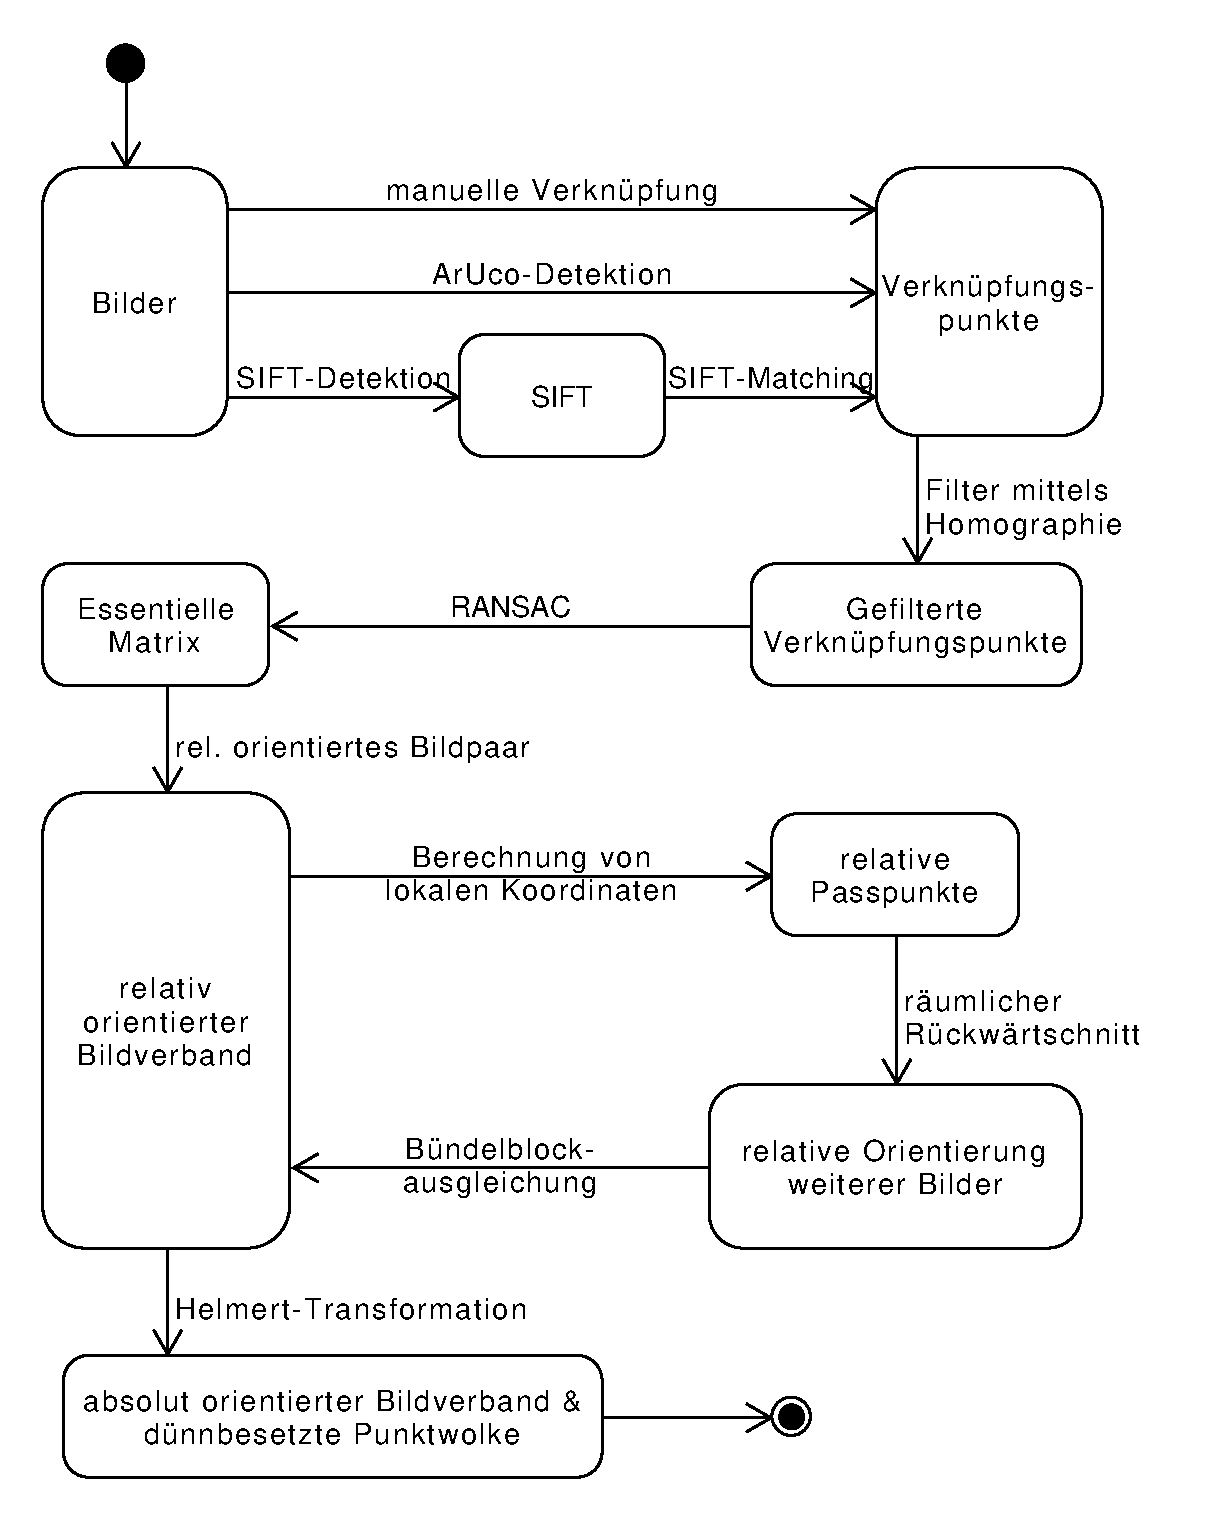
\includegraphics[width=0.8\textwidth]{./img/Ablauf.pdf}
    \centering
    \caption{Ablauf der Bildverknüpfung, nach \citealt[S. 492]{luhmann}} %Bildunterschrift
    \label{img:ablauf} %ID fürs Bild
\end{figure}

\section{Innere Orientierung}
\label{s:innereorientierung}
Aus der Position eines Punktes in einem Bild kann vereinfacht gedacht ähnlich einer Messung mit einem Theodolit die Richtung des Punktes in Relation zu der Kamera bestimmt werden. Damit diese Berechnung möglich wird, müssen die Parameter der Kamera bekannt sein, die sogenannte innere Orientierung. Sie beschreibt die Abbildung der Kamera mathematisch. Wichtigste Parameter sind hierbei die Lage des Bildhauptpunktes und die Kamerakonstante. Außerdem zählen hierzu auch die Parameter, die die Bildfehler wie die Verzeichnung, beschreiben. \citep[S. 179f]{luhmann}

Die innere Orientierung kann während der Messung beispielsweise mittels Bündel\-block\-ausgleichung bestimmt werden. Bedingung hierfür ist jedoch, dass die innere Orientierung stabil ist und sich nicht während der Messung ändert \citep[S. 181f]{luhmann}.

Jede Einstellung der Kameraoptik verändert die innere Orientierung und auch jede Kamera,auch einer Modellreihe, kann je nach Genauigkeitsanspruch als unterschiedlich angesehen werden. Änderungen können sich beispielsweise durch Umfokussierung oder die Nutzung eines optischen Zoom ergeben, aber auch durch einen mechanisch instabilen Aufbau der Kameras. Daher sollten die Bilder möglichst mit einer Kamera mit festen Einstellungen (Brennweite, Fokus, Blende, Objektiv) aufgenommen werden. Änderungen der Empfindlichkeit (ISO-Zahl) oder Belichtungszeit sind unproblematisch für die innere Orientierung \citep[S. 176]{luhmann}.


\section{Bilder}
\label{s:bilder}

Die Berechnung der Tiefeninformationen ist nur möglich, sofern der Punkt in mindestens einem weiteren Bild abgebildet ist. Die Genauigkeit der Berechnung ist vom Schnittwinkel dieser beiden Strahlen abhängig. Um möglichst gute Schnitte zur Ver\-fügung zu haben und die innere und äußere Orientierung möglichst gut berechnen zu können, müssen diese Bilder einige Bedingungen erfüllen.

\subsubsection{Überlappung und Bildinhalte}
Da die Bilder durch identische Punkte verbunden werden, müssen die Bildinhalte sich überlappen. Die automatische Identifikation von identischen Punkten ist auf verschiedene Weisen möglich: Entweder durch die Nutzung von codierten Passpunkten wie ArUco-Markern oder konzentrischen Passpunkten nach \cite{schneider}. Alternativ können auch eine Merkmalsextraktion zur Indentifikation von gemeinsamen Punkten genutzt werden, beispielsweise durch die SIFT-Methode. Hierfür muss die oberfläche aber genügend Texturen aufweisen. \citep[S. 478]{luhmann}

\subsubsection{Belichtung}
und bei sich stark ändernden Helligkeitsverhältnissen auch hilfreich, jedoch wird hierdurch auch die Helligkeit der Verknüpfungspunkte verändert, was wiederum problematisch sein kann. Entsprechend ist es empfehlenswert bei gleichmäßiger Beleuchtung, die sich auch nicht ändern sollte, die Bilder zu erstellen - also beispielsweise bei bedeckten Himmel.

\subsubsection{Position und Ausrichtung der Kamera}
Bilder, die vom gleichen Standpunkt aufgenommen wurden, sind oft nur ungenau verknüpfbar. Daher empfiehlt es sich, eher um Objekte herum zu gehen, statt beispielsweise bei Innenräumen sich nur in die Mitte zu stellen und sich zu drehen. Während der Aufnahmen sollte die Kamera natürlich möglichst ruhig gehalten werden, um möglichst scharfe Bilder zu generieren. Dies ist vor allem bei UAV-Flügen relevant, die auch aus hoher Geschwindigkeit Bilder aufnehmen könnten. Jedoch weisen die meisten Digitalkamera einen Rolling-Shutter-Effekt auf, dass heißt die Bildreihen werden nicht alle zeitgleich aufgenommen, sondern die oberen vor den unteren. Daher ist es sinnvoll, das UAV kurz schweben zu lassen und dann ein Bild zu machen. \citep[S. 147]{opendronemap}

Umso weiter die Kamera vom Objekt entfernt ist, umso mehr Inhalte und entsprechend mehr Verknüpfungsmöglichkeiten sind im Bild enthalten. Daher sollte sich immer klar gemacht werden, welche Auflösung benötigt wird und entsprechend die Entfernung bzw. bei UAV-Aufnahmen die Höhe zu wählen. Der Abstand sollte außerdem variiert werden, da dieses bei der Ausgleichung der inneren Orientierung hilft. \citep[S. 144f]{opendronemap}

\subsubsection{Schärfentiefe und Fokussierung}


\section{Verknüpfungspunkte}
Um die einzelnen Bilder verknüpfen zu können, werden identische Punkte zwischen zwei oder mehr Bildern benötigt. Diese können klassisch per Hand erfasst werden, jedoch ist dieses schon bei kleineren Projekten sehr zeitaufwändig. Daher wurde zusätzlich die Möglichkeit genutzt, automatisch Verknüpfungspunkte zu erzeugen.

\subsection{ArUco-Marker}
Eine Variante der automatischen Verknüpfungspunkte sind die sogenannten ArUco-Marker. Diese werden häufig für die Orientierung bei Augmented-Reality-Anwend\-ungen genutzt. OpenCV unterstützt die Erkennung dieser Marker. Sie werden als codierte Messmarken verwendet und können automatisch im Subpixelbereich erkannt werden. Jede Ecke kann hier einzeln identifiziert werden, sodass ein erkannter Marker vier Verknüpfungspunkte liefern kann.

\subsection{SIFT}
Die SIFT-Methode liefert Verknüpfungspunkte aus Mustern auf den photographierten Oberflächen. Es ist meist nicht notwendig explizit Marker an dem aufzunehmenden Objekt anzubringen, sofern seine Oberfläche nicht strukturlos ist (glatte weiße Wände etc.) oder in Bewegung ist.

Zur Erkennung von Merkmalen setzt das Verfahren auf die Detektion von Kanten. Diese werden in verschiedenen Stufen einer Bildpyramide erkannt und ihre Extrema berechnet. Es werden diese Merkmale weiter ausgedünnt, beispielsweise über den Kontrast. Sofern ein möglicher Marker identifiziert wurde, wird eine Beschreibung erzeugt. Diese erfolgt  durch Analyse der Helligkeitsabweichungen zu den Nachbar-Pixeln und wird an der stärksten Abweichung ausgerichtet. Hierdurch wird die Beschreibung dann richtungsunabhängig. Mit diesen kann dann die Übereinstimmung von zwei Markern in zwei Photos bestimmt werden, auch wenn die Bilder zueinander gekippt oder gedreht sind.
\citep[S. 483]{luhmann4}

\section{Verknüpfung von Bildern}
\label{s:photogramm}
Durch die drei beschriebenen Verfahren und die hieraus entstandenen Verknüpfungs\-punkte können die Bilder miteinander verknüpft werden. Da durch GNSS nur eine sehr grobe und ggf. auch falsche Vorausrichtung besteht, kann diese nur als sehr grobes Hilfsmittel genutzt werden. In diesen Ansatz wird es nur für die Beschränkung der SIFT-Detektion auf Bilder, die nahe beieinander sind oder sich ArUco- oder manuelle Punkte teilen, genutzt.
Für die eigentliche Verknüpfung werden dann nur photogrammmetrische Verfahren genutzt. Über diese wird im Folgenden ein kurzer Überblick gegeben.

\begin{comment}
\subsection{Homographie}
grobe Filterung
\end{comment}

\subsubsection{Abbildungsgleichung}
\label{ss:abbildungsgleichung}
Die Abbildung eines Punktes auf einem Bild wird durch die Abbildungsgleichung beschrieben. In der Matrizenrechnung ergibt sich dieser aus der Multiplikation mit der Projektionsmatrix $P$. Diese ergibt sich aus der Kameramatrix $K$, der Rotation $R$ und dem Projektionszentrum $X_0$. (siehe \autoref{abbildungsgleichung}, nach \citealp[S. 244]{hartley} und \citealp[S. 288]{luhmann4})

\begin{align}
    \label{abbildungsgleichung}
    x' & = P \cdot X       \\
    P  & = K \cdot [R|X_0] \\
    P  & =
    \begin{bmatrix}
        c_x & 0   & x'_0 \\
        0   & c_y & y'_0 \\
        0   & 0   & 1
    \end{bmatrix}
    \cdot
    \begin{bmatrix}
        r_11 & r_21 & r_31 & X_0 \\
        r_12 & r_22 & r_32 & Y_0 \\
        r_13 & r_23 & r_33 & Z_0 \\
    \end{bmatrix}
\end{align}

Um die Beziehung zwischen zwei Bildern aufzustellen, kann man die Abbildungsgleichung nutzen. Da es hier nur um die Beziehung zwischen zwei Bildern geht, kann die Rotation und Translation des ersten Bildes auf 0 gesetzt werden ($R$ ist dann eine 3x3-Einheitsmatrix und $X_0$ ein Nullvektor). $X_0$ des zweiten Bildes wird zur Translation zwischen den beiden Bildern. \citep[S. 326]{luhmann4}

\subsubsection{Fundamental-/Essentielle Matrix}
Die Fundamentalmatrix beschreibt das Verhältnis von identischen Punkten in zwei Bildern zueinander. Sie kann genutzt werden, um die Drehung und Verschiebung zwischen zwei Aufnahmeorten zu bestimmen. Die Formel für die Fundamentalmatrix lautet:
\begin{align}
    x'^T \cdot F \cdot x'' & = 0
\end{align}
Sie unterscheidet sich nur von der Essentiellen Matrix in der Eigenschaft, dass bei der Essentiellen Matrix die Kameraparameter bekannt sein müssen. Diese werden dann auf die Bildkoordinaten angewendet und $x'$ und $x''$ werden so unabhängig (normalisiert) von den Kameraeinstellungen. Mittels Singulärwertzerlegung lässt sich dann die Rotation und Translation aus der Essentiellen Matrix bestimmen. Im Falle von Bildern die mit Digitalkameras aufgenommen wurden sind die Kameraparameter zumindest näherungsweise aus den EXIF-Daten der Bilder bekannt, sodass dieser Weg hier genutzt werden kann. \citep[S. 257]{hartley}

In der entstandenen Software wurde die Methode verwendet, um die Verknüpfung des Startpaares zu errechnen.

\subsection{Fundamental-/Essentielle Matrix}
Die Fundamentalmatrix beschreibt das Verhältnis von identischen Punkten in zwei Bildern zueinander. Sie kann genutzt werden, um die Drehung und Verschiebung zwischen zwei Aufnahmeorten zu bestimmen. Die Formel für die Fundamentalmatrix lautet:
\begin{align}
    x'^T \cdot F \cdot x'' & = 0
\end{align}
Sie unterscheidet sich nur von der Essentiellen Matrix in der Eigenschaft, dass bei der Essentiellen Matrix die Kameraparameter bekannt sein müssen. Diese werden dann auf die Bildkoordinaten angewendet und $x'$ und $x''$ werden so unabhängig (normalisiert) von den Kameraeinstellungen. Mittels Singulärwertzerlegung lässt sich dann die Rotation und Translation aus der Essentiellen Matrix bestimmen. Im Falle von Bildern die mit Digitalkameras aufgenommen wurden sind die Kameraparameter zumindest näherungsweise aus den EXIF-Daten der Bilder bekannt, sodass dieser Weg hier genutzt werden kann. \citep[S. 257]{hartley}

In der entstandenen Software wurde die Methode verwendet, um die Verknüpfung des Startpaares zu errechnen.

\subsection{Vorwärtsschnitt}
Aus den zwei Projektionsmatrizen zweier Bilder und der Position eines identischen Punktes in beiden Bildern lassen sich dann lokale (Modell-)Koordinaten des Punktes berechnen. Da auch dieses nicht fehlerfrei ist, wurde hierfür die Methode der linearen Triangulation verwendet. Hierbei wird der entstehende Fehler ausgeglichen. \citep[S.312]{hartley}

\subsection{Rückwärtsschnitt}
Entsprechend lässt sich auch aus der Position von Punkten mit bekannten lokalen Koordinaten die Position und Drehung eines Bildes berechnen. Dieses wurde genutzt, um weitere Bilder an das Startpaar heranzuknüpfen. Hierfür werden mindestens 5 Punkte benötigt. \citep[S. 533ff]{hartley}


\section{Bündelblockausgleichung}
Mittels Bündelblockausgleichung können die grob mit den vorher genannten Verfahren bestimmten Positionen und Drehungen in einer Ausgleichung optimiert werden. Hierzu gehen alle Parameter der Bilder und die Positionen der Passpunkte in die gemeinsame Ausgleichung ein. Grundlage der Ausgleichung ist die in \autoref{ss:abbildungsgleichung} beschriebene Abbildungsgleichung. Als Ergebnis erhält man die ausgeglichenen Parameter und Genauigkeitsangaben für diese. \citep[S. 340]{luhmann4}

\chapter{Aufbau des Messsystemes}
Die Kameras sollten eine höhe geometrische Auflösung und möglichst stabile innere Orientierung aufweisen. Außerdem sollen sie während einer Messkampagne nicht in ihrer Lage zueinander verändert werden, damit die äußere Orientierung größtenteils unverändert bleibt. Daher ist ein stabiler Rahmen notwendig, an welchem die Kameras verdrehsicher angebracht werden können. Kleinere Restfehler in den Orientierungen können mit ausgeglichen werden.
Um Ungenauigkeiten durch Bewegungen zu verhindern, müssen die Kameras möglichst zeitgleich auslösen. Daher ist eine gemeinsame Steuerung und Kommunikation zwischen den Kameras notwendig. Außerdem sollen alle Bilder dann auf das Steuerungssystem übertragen werden, hierfür wir eine Form der Datenübertragung benötigt. Damit die Bilder möglichst schattenfrei ausgeleuchtet werden, muss Beleuchtung mit eingeplant werden. Außerdem muss die Stromversorgung der einzelnen Kameras sichergestellt sein.

Aus diesen Anforderungen ergeben sich die einzelnen Abschnitte dieses Kapitels.

\section{Kameras}
Als Kameras wurde das Raspberry Pi Camera Module 3 verwendet, welches jeweils von einem Raspberry Pi Zero W gesteuert wird. Im Vergleich zu anderen günstigen Kameras wie Webcams oder der ESP32 CAM haben die Kameras eine hohe geometrische Auflösung von 12 Megapixeln und dennoch mit $1,4~\mu m$ relativ große Pixel \citep{raspi_cam_datasheet}, was im subjektiven Eindruck eine sehr gute Bildqualität ergibt.

Nachteil und Vorteil zugleich ist, dass die Kamera über einen Autofokus verfügt, der aber auch elektronisch gesteuert manuell fokussieren kann. Dieser verschlechtert die Stabilität der inneren Orientierung (vgl. \autoref{s:innereorientierung}) weiter und wurde daher auch besonders im \todo{Verweis zu Fokusexperimenten} analysiert. Da die Bilder aber Nahbereich zwischen $20$ und $70~\text{cm}$ benötigt werden, ist hier die Schärfentiefe niedrig. Der elektronische Fokus, eine wiederholgenaue und damit mathematisch modellierbare Fokussierung vorausgesetzt, ermöglicht hier, Fokusstacking zu nutzen um den Schärfebereich zu vergrößern.

Weiterer Vorteil der Lösung mit einzelnen Raspberry Pis ist es, dass hierdurch bereits die einzelnen Kameraeinheiten Berechnungen wie das Identifizieren von Passpunkten übernehmen könnten und auch durch die Nutzung von Netzwerkverbindungen für die Steuerung das System skalierbar im Sinne der Anzahl der Kameras aber auch der Größenordnung der Abstände zwischen den Kameras.

\section{Rahmen}
Der Rahmen muss möglichst stabil sein, damit die Kameras sich nicht in ihrer Lage verändern können. Jedoch sollte das System auch weiterhin transportabel - also nicht zu schwer - und veränderbar bleiben, beispielsweise Kameras für Messreihen in ihrer Lage verändert werden. Der Aufbau aus genormten Bauteilen bietet sich an, um hier ggf. den Nachbau einfach ermöglichen zu können.

Als mögliche Materialien kamen Holz, Stahl und Aluminum in Frage. Aufgrund der einfachen Bearbeitung und der genormten Profile, wurde sich für Aluminiumprofile entschieden. Diese gibt es in verschiedenen Ausführungen mit Nuten an den Seitenflächen, so dass eine einfache Montage, aber auch eine Demontage zu Transportzwecken, möglich wird. Außerdem sind diese sehr stabil bei leichtem Gewicht.

Durch eine Konstruktion mit Eckwürfeln sowie dem Einbau von dreieckigen Strukturen und Platten, die Scheibenwirkung haben, wurde die Stabilität der Verbindungen erhöht.

\section{Beleuchtung}
Um möglichst gute Bilder zu erzeugen, sollte das Objekt gut ausgeleuchtet sein. Eine dunkle Umgebung verlängert die Belichtungszeit, wodurch die Gefahr von unscharfen Aufnahmen steigt und dunklere Bereiche (ungleichmäßige Ausleuchtung) verursacht Rauschen in diesen Bildbereichen. Daher soll das System eine gleichmäßige Ausleuchtung ermöglichen. Problematisch ist hierbei, dass die Kameras ggf. auch die Lichtquellen mit im Bildbereich haben können, wodurch Linsenreflexionen oder Ausbrennen der Bildbereiche möglich sind.

Es wurde sich zur Beleuchtung für einzeln steuerbare LED-Lichtstreifen entschieden. Diese können einfach an den Aluprofilen montiert werden und ermöglichen es, einzelne Bereiche und so ggf. blendende Bereiche abzuschalten.

\section{Stromversorgung}
Die Raspberry Pis werden mit 5~Volt betrieben. Der Raspberry Pi Zero mit Kamera hatte dabei in Messungen einen maximalen Stromverbrauch von 270~mA aufgezeigt, der Raspberry Pi 4 kann bis zu 1,5~A unter Last verbrauchen. Hieraus ergibt sich ein Gesamtstromverbrauch von maximal rund 8~Ampere. Für den Raspbery Pi 4 wurde ein eigenes Netzteil eingeplant und für die Zero W ein gemeinsames 35 Watt-Netzteil. Versuche zeigten jedoch, dass der Stromverbrauch kurzfristig höher ausfallen konnte, so dass die Zero W, die am meisten von Spannungsabfällen betroffen sind zum Absturz gebracht wurden, wenn alle Kameras gleichzeitig auslösten. Nach dem die Last auf sicherheitshalber auf zwei weitere Netzteile verteilt wurde, lief das System zuverlässig.

Als Kabelmaterial wurde Klingeldraht mit $0,75~\text{mm}^2$ verwendet. Der relativ hohe Kabelquerschnitt soll für einen geringen Spannungsabfall sorgen. Durch die Verwendung von mehreren Netzteilen ist dieser jedoch nun nicht mehr notwendig. Hier würde sich nun ein geringerer Querschnitt anbieten, auch um eine einfachere Verbindung zu den Raspberry Pi Zero W zu ermöglichen. Diese wurden auf Seiten der Zero W verlötet und in den Verteilerdosen mit Federkraftklemmen verbunden.

Die Stromversorgung der Beleuchtung erfolgt über ein 12-V-Netzteil mit $3,5~\text{A}$ Ausgangsleistung. Auch hier wurde Klingeldraht zur Verteilung zwischen den einzelnen Holmen genutzt.

Beim WLAN-Router war ein entsprechendes USB-Netzteil mitgeliefert.

\section{Kommunikation und Datenübertragung}
Die Kommunikation zwischen den Raspberry Pis erfolgt über WLAN. Vorteil dieser Lösung ist, dass hier keine weiteren Leitungen außer der Stromversorgung zu den einzelnen Raspberry Pi Zero W benötigt wird und es auch möglich wäre, die gleiche Hard- und Software auch für ein größeres System ohne Änderungen zu nutzen. Nachteilig ist die Verbindungsgeschwindigkeit, gerade im Hinblick auf die Synchronisierung der Kameras. Diese Problematik soll aber durch entsprechende Programmierung der Software möglichst klein gehalten werden.

Als weitere Datenleitungen wird eine Steuerleitung für die LED-Streifen benötigt. Über diese erfolgt die Steuerung der einzelnen LED-Gruppen. Auch hier wurde wieder Klingeldraht verwendet.

\chapter {Software-Entwicklung}
Für die Steuerung der Kameras und die anschließende Berechnung des 3D-Modelles muss ein Betriebssystem für das Kamerasystem und eine entsprechende Schnittstelle zu einer SfM-Software geschaffen werden. Diese Entwicklung erfolgte hauptsächlich in Python in Form von Prototyping. Das Kapitel beschreibt die Anforderungen an die Software in \autoref{sec:Anforderungsanalyse}. Anschließend werden hieraus die Anwendungsfälle (\autoref{sec:Anwendungsfallmodellierung}) erarbeitet und abschließend die Implementation (\autoref{sec:Implementierung}) beschrieben.

\section{Anforderungsanalyse}
\label{sec:Anforderungsanalyse}

\subsection{Funktionale Anforderungen}
\begin{itemize}
    \item Die Kameras sollen zeitgleich auslösbar sein. Die Auslösung soll möglichst ver\-zögerungs\-frei erfolgen.
    \item Die Steuerung soll auch unabhängig von anderen Geräten möglich sein, beispielsweise per Tastensteuerung.
    \item Der Status des Systemes soll für den Nutzer erkennbar sein - auch ohne Anschluss eines Computers etc..
    \item Es sollen Passpunkte automatisch gefunden und und für die Bestimmung der äußeren Orientierung genutzt werden.
    \item Die Bilder sollen scharf und fokussiert sein.
\end{itemize}

\subsection{Schnittstellen}
\begin{itemize}
    \item Die Daten sollen intern gespeichert werden.
    \item Eine Speicherung auf tragbaren Speichermedien wie USB-Sticks soll möglich sein.
    \item Eine direkte Übertragung an SfM-Software soll möglich sein.
\end{itemize}

\subsection{Nicht-funktionale Anforderungen}
\begin{itemize}
    \item Die Erfassung soll ohne weitere Hardware möglich sein. Das System soll unabhängig von Netzwerkanschlüssen etc. sein.
    \item Alle Kommunikation soll über WLAN erfolgen.
\end{itemize}

\section{Anwendungsfallmodellierung}
\label{sec:Anwendungsfallmodellierung}

Entsprechend der benötigten Schritte aus \autoref{c:photogrammmetrie} und \autoref{img:ablauf} wurde die Anwendungsfälle, die die Benutzeroberfläche ermöglichen soll, im Anwendungsfall-Dia\-gramm in \autoref{img:anwendungsfall} zusammengetragen.

\begin{figure}[!htbp]
    \centering
    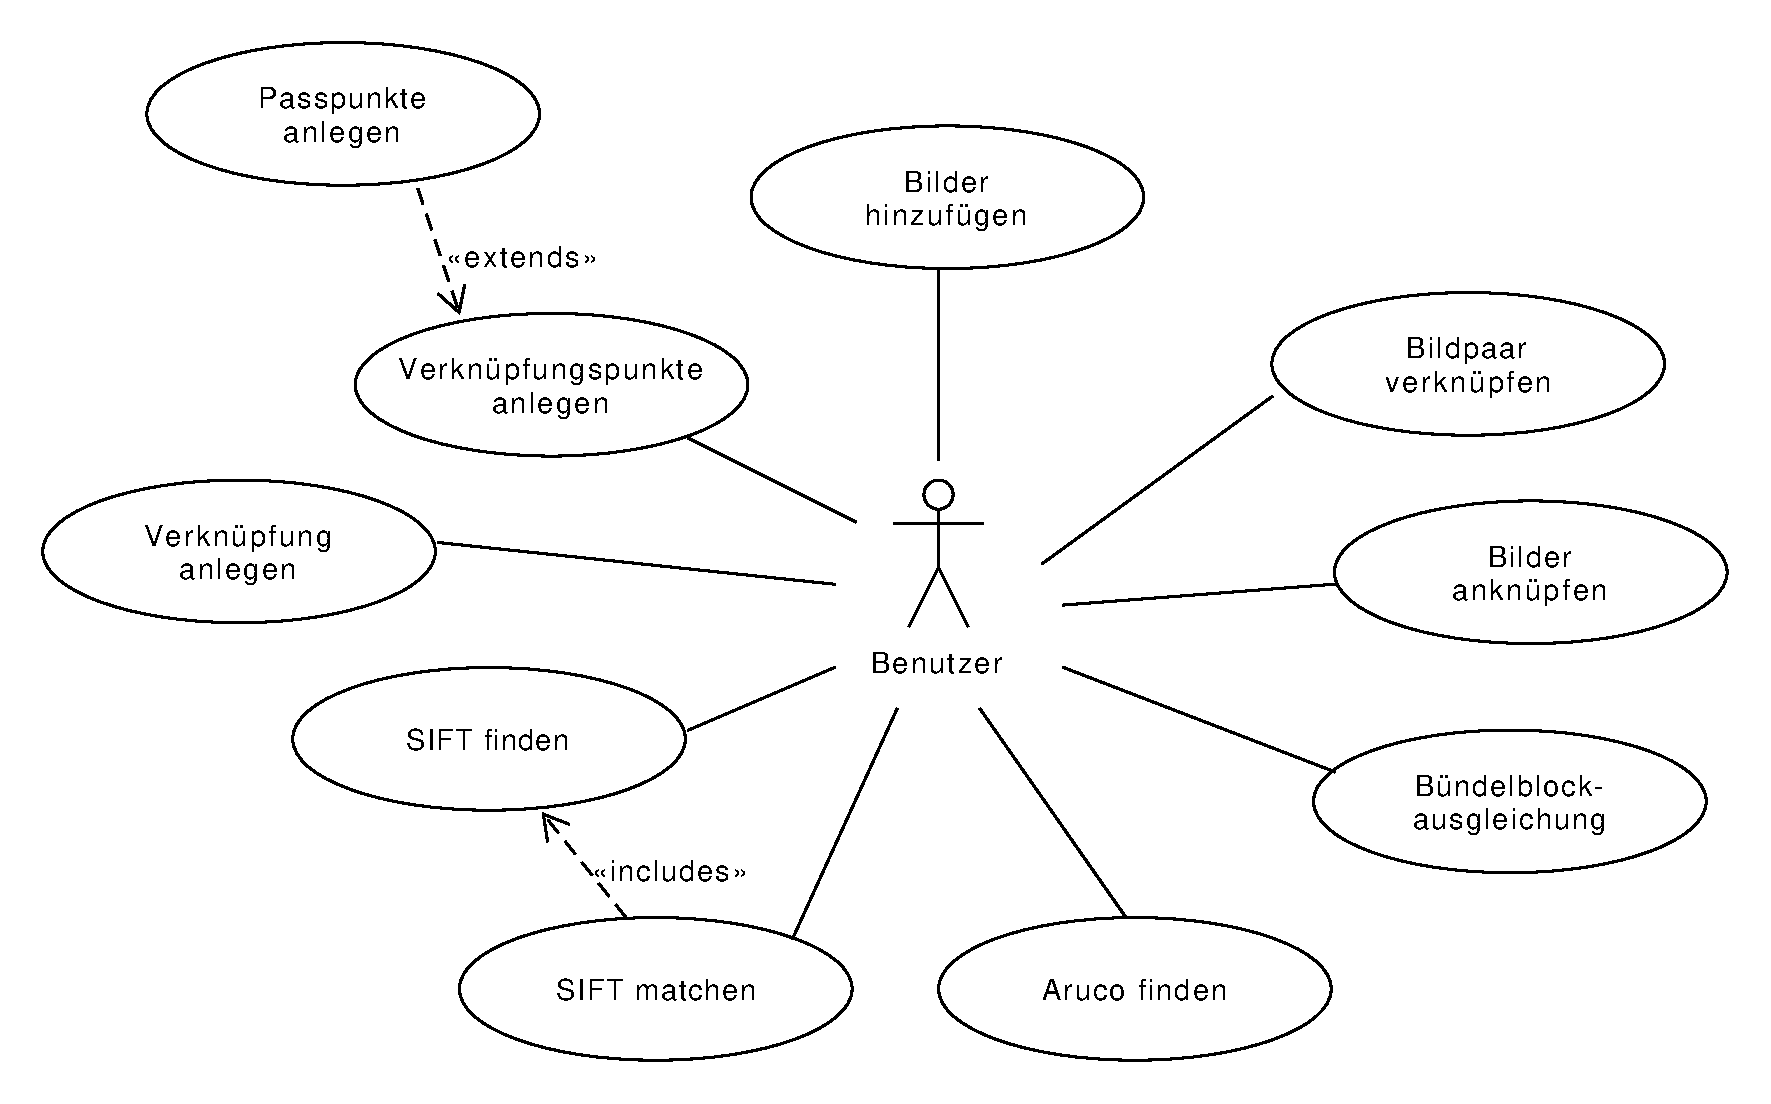
\includegraphics[width=1\textwidth]{./img/UseCase.pdf}
    \centering
    \caption{Anwendungsfall-Diagramm} %Bildunterschrift
    \label{img:anwendungsfall} %ID fürs Bild
\end{figure}

Aus den benötigten Daten wurde das Domänen-Klassendiagramm aus \autoref{img:dokladia} erzeugt. Dieses zeigt vor allem die Abhängigkeiten der einzelnen Datensätze untereinander.

\begin{figure}[!htbp]
    \centering
    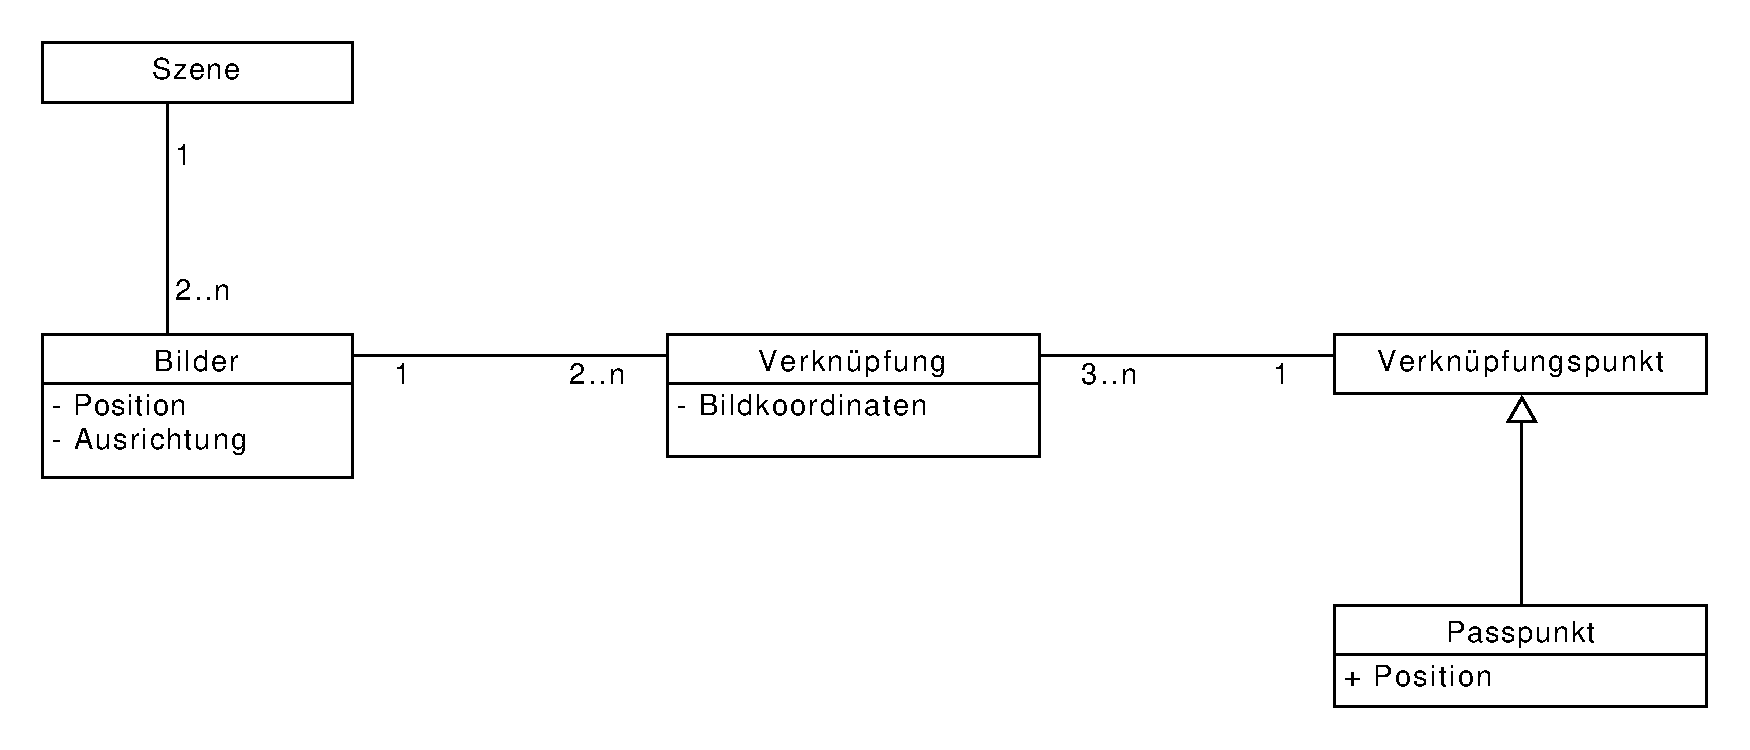
\includegraphics[width=1\textwidth]{./img/DomaenenKlassendiagramm.pdf}
    \centering
    \caption{Domänen-Klassendiagramm} %Bildunterschrift
    \label{img:dokladia} %ID fürs Bild
\end{figure}

\section{Implementierung}
\label{sec:Implementierung}
Dieses ist dann auch Grundlage für die Implementierung der SQLite-Datenbank. Der Datenbankaufbau ist \autoref{img:datenbank} zu entnehmen. Die Datenbank dient der Zwischenspeicherung der Passpunkte und der durchgeführten Berechnungen.

\begin{figure}[!htbp]
    \centering
    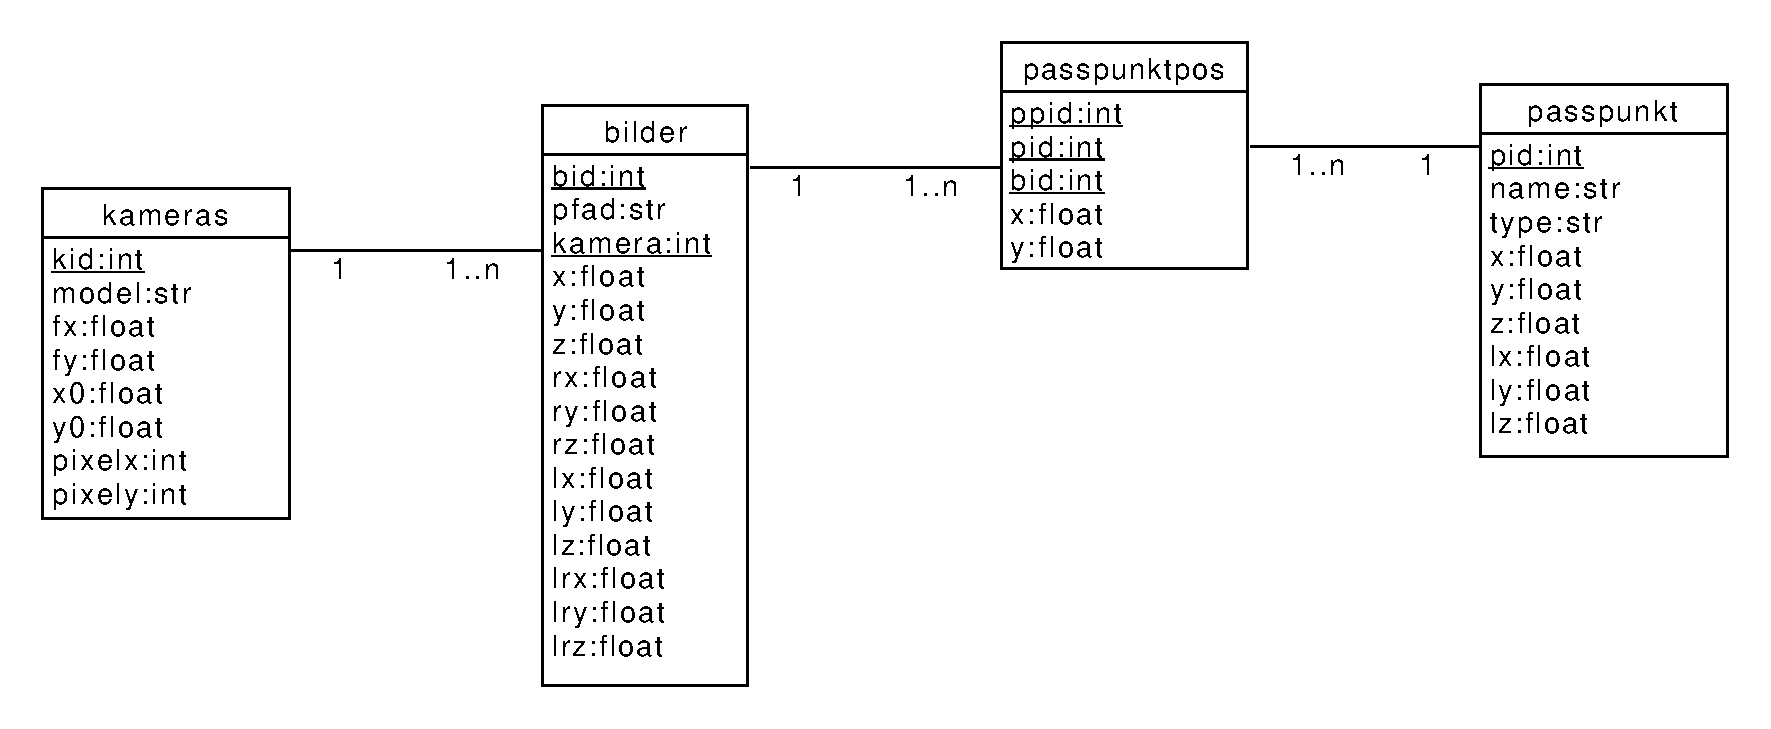
\includegraphics[width=1\textwidth]{./img/datenbank.pdf}
    \centering
    \caption{Datenbank-Struktur} %Bildunterschrift
    \label{img:datenbank} %ID fürs Bild
\end{figure}

Das Backend wurde in Python entwickelt. Die Pakete orientieren sich an den Arbeitsschritten aus dem Ablaufdiagramm (\autoref{img:ablauf}). Die einzelnen Python-Module greifen auf die oben beschriebene SQLite-Datenbank zu. Die einzelnen Module sind der Übersicht in \autoref{img:python} zu entnehmen.

\begin{figure}[!htbp]
    \centering
    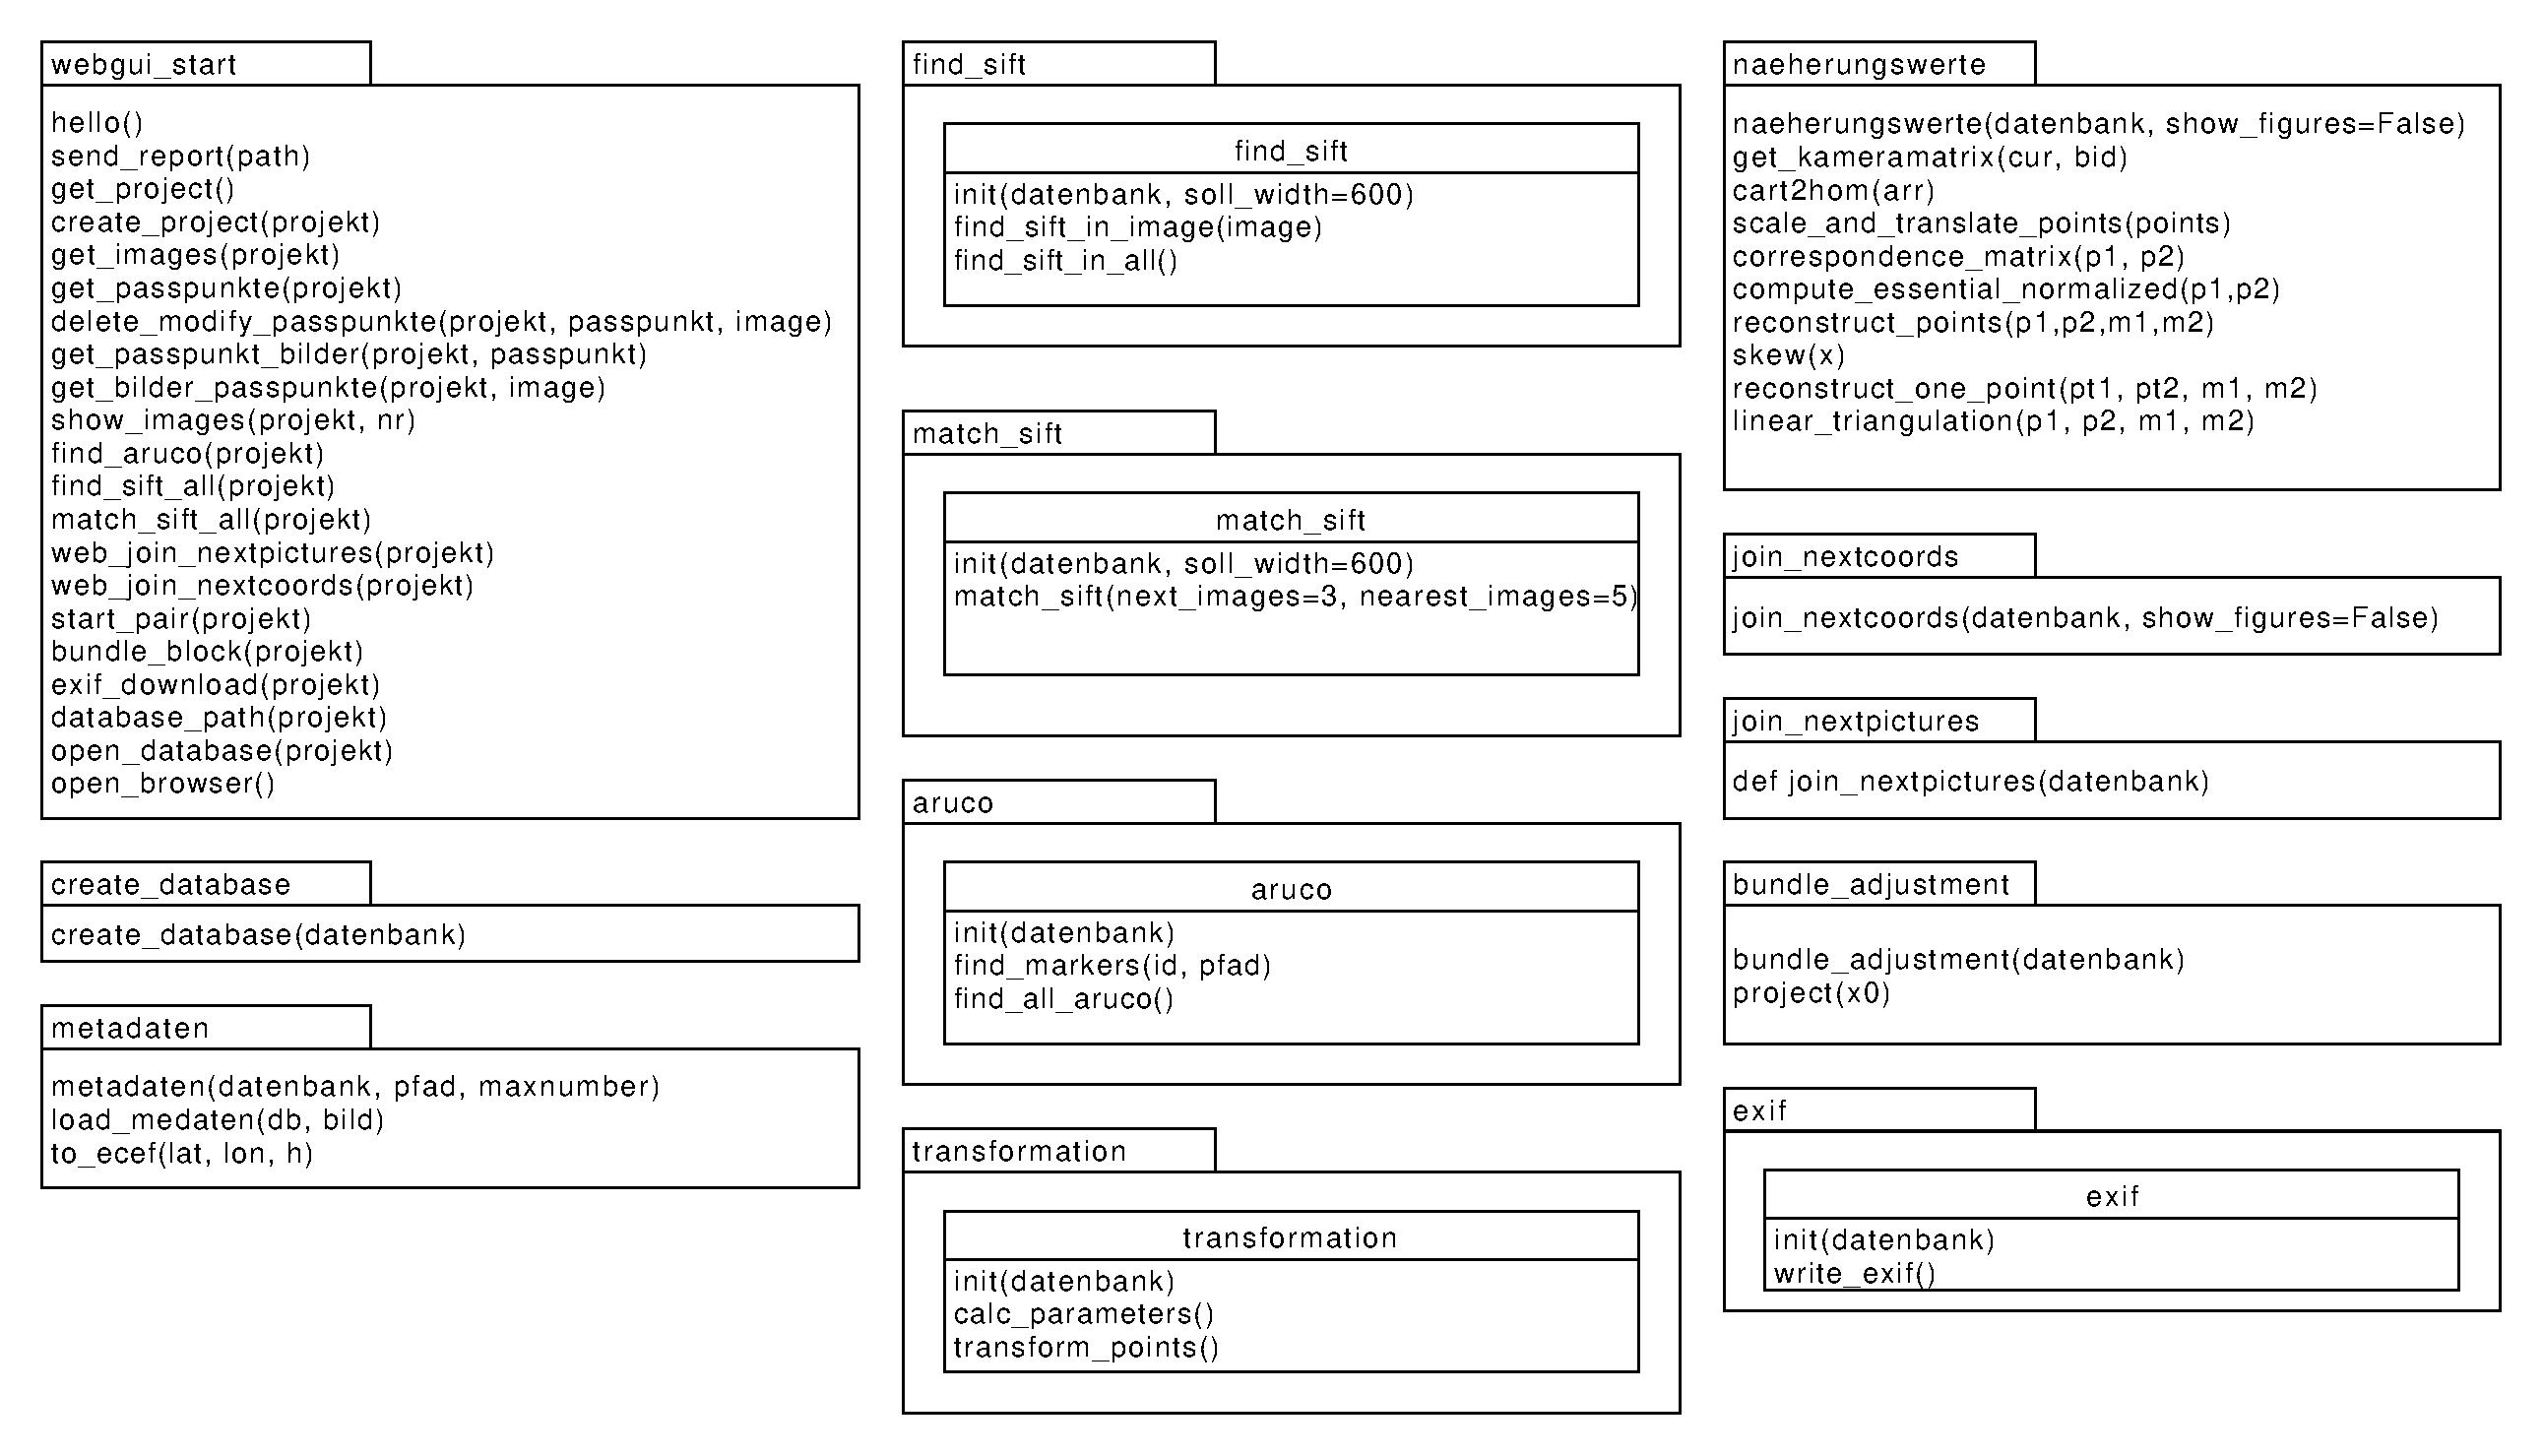
\includegraphics[width=1\textwidth]{./img/python.pdf}
    \centering
    \caption{Implementierung der Python-Pakete} %Bildunterschrift
    \label{img:python} %ID fürs Bild
\end{figure}

Über das Webstart-Modul werden dann die einzelnen Module über eine Website mit TypeScript angesprochen. Die einzelnen TypeScript-Klassen sind der \autoref{img:typescript} zu entnehmen. Hierbei wurde darauf Wert gelegt, die einzelnen Funktionen modular zu halten, sodass die Möglichkeit besteht, das System mit weiteren Modulen zu erweitern.

\begin{figure}[!htbp]
    \centering
    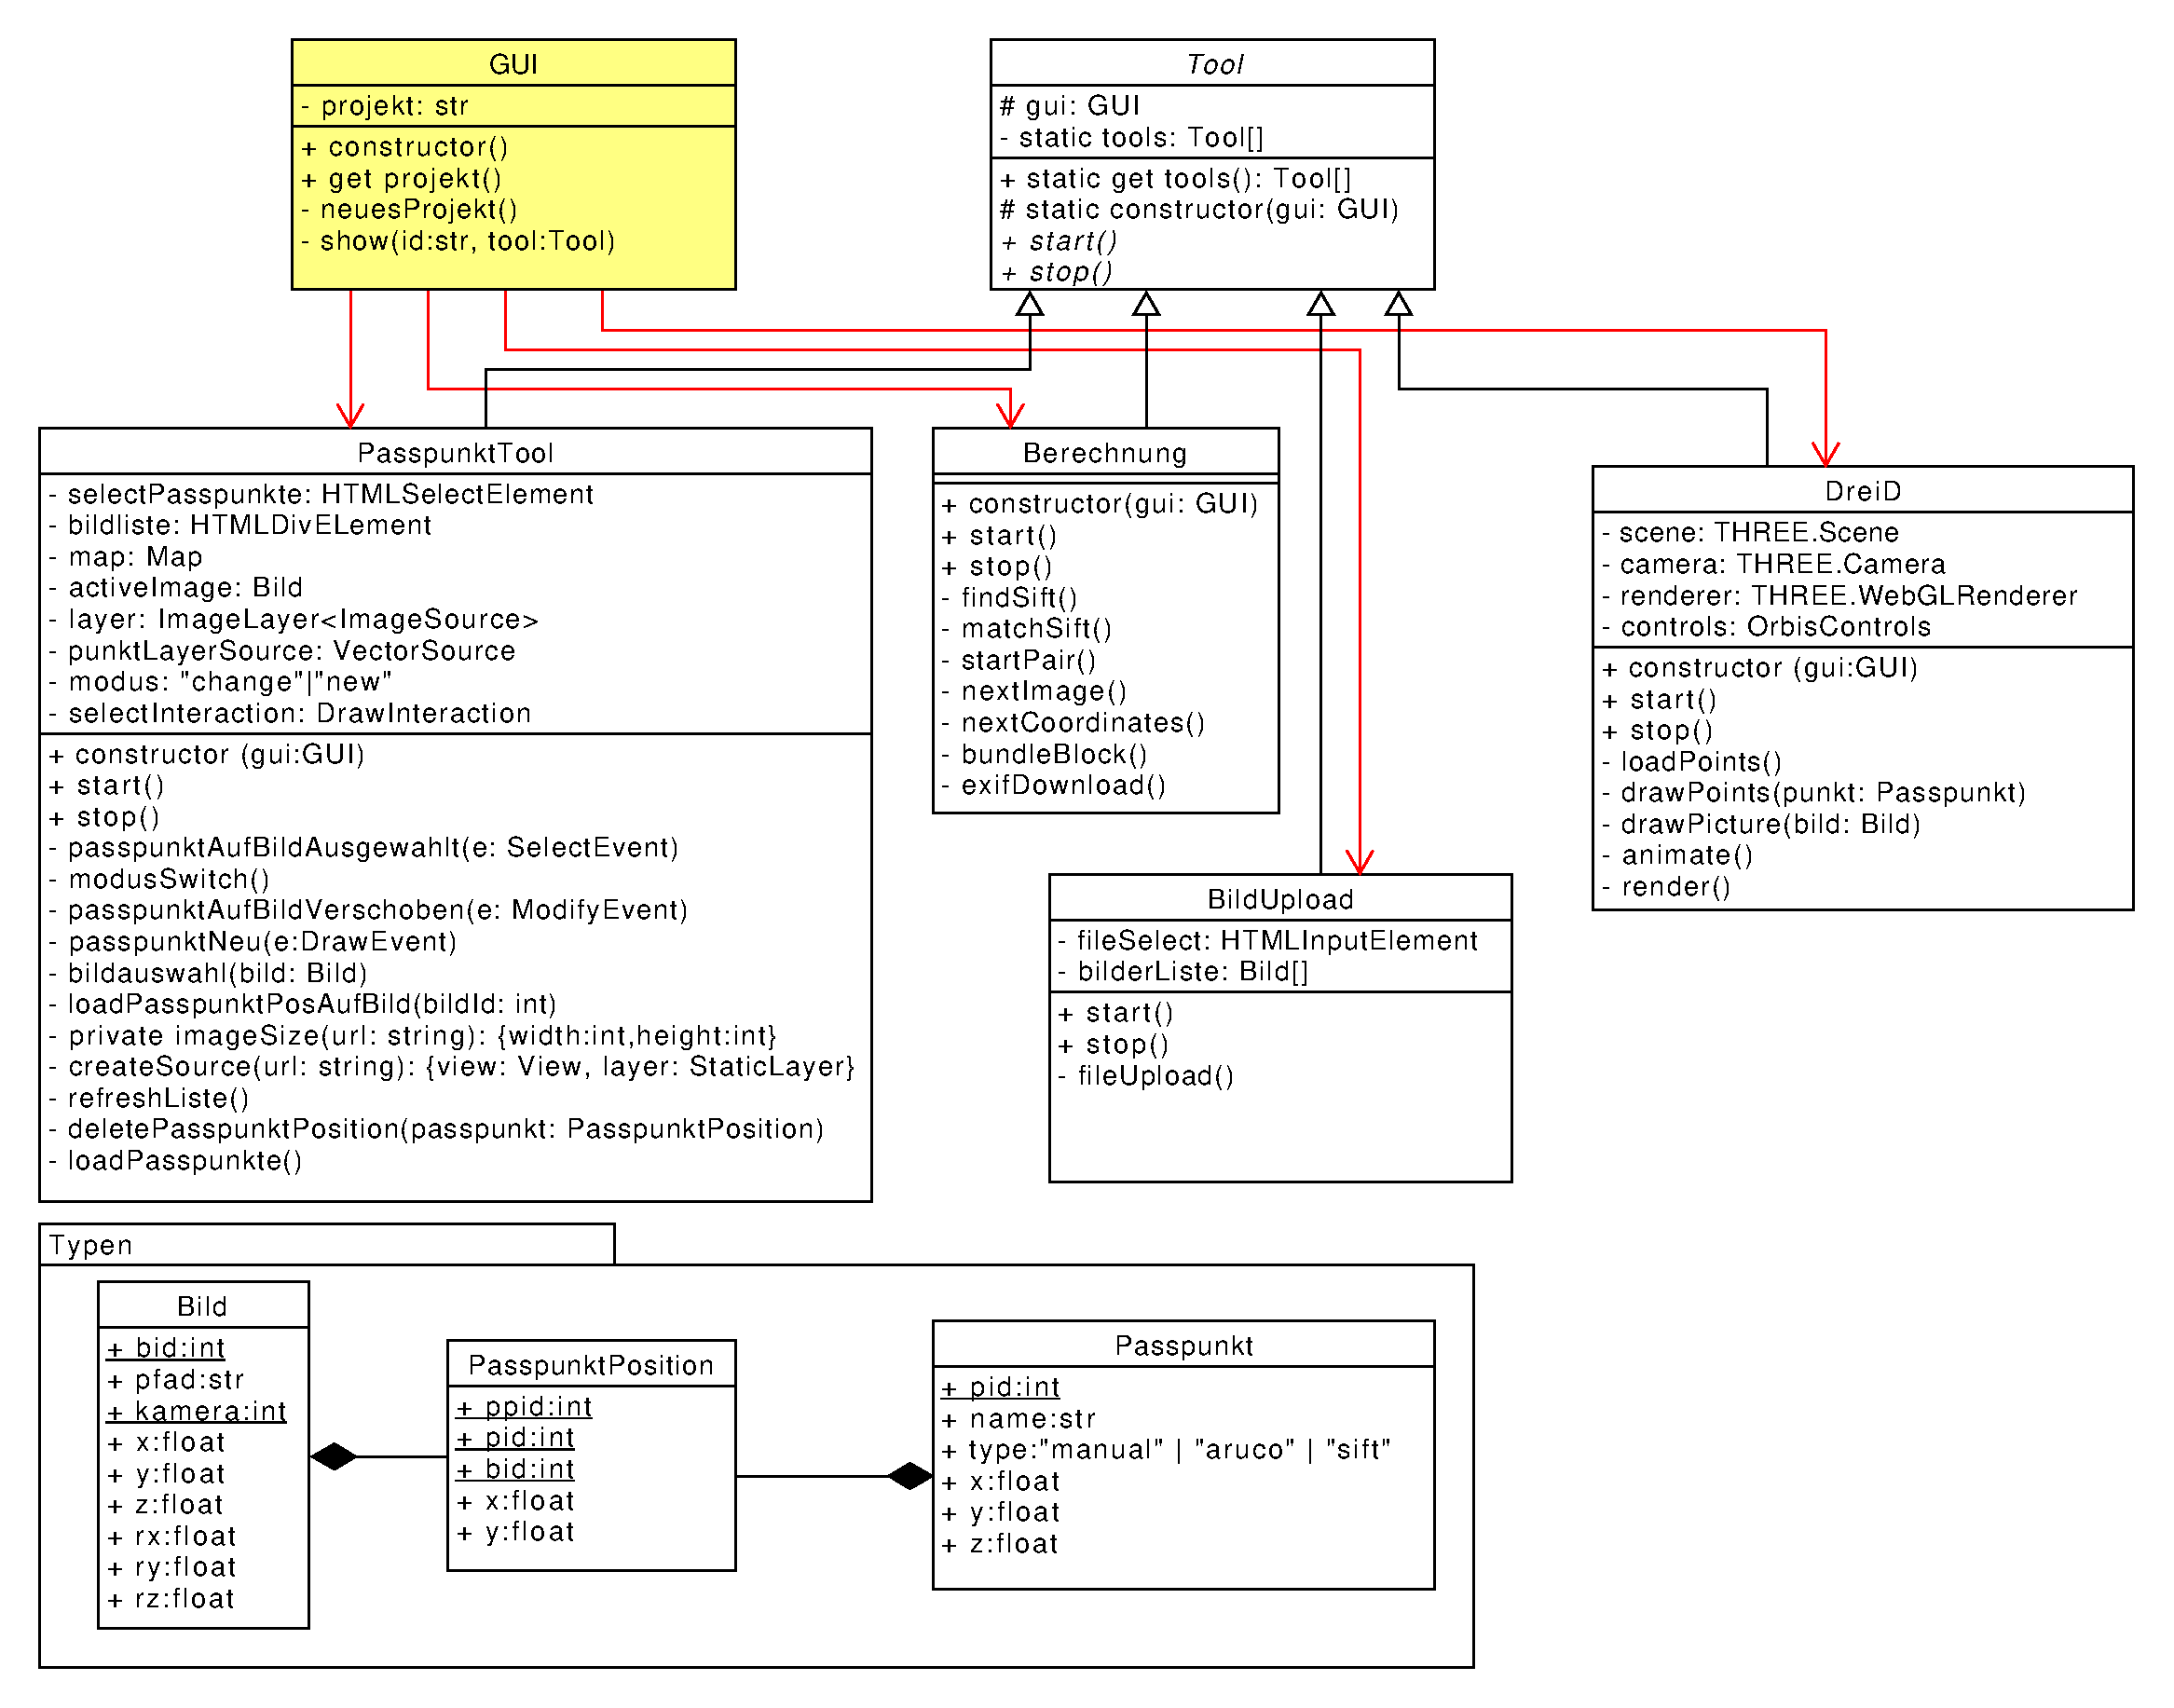
\includegraphics[width=1\textwidth]{./img/typescript.pdf}
    \centering
    \caption{Implementierung der TypeScript-Klassen} %Bildunterschrift
    \label{img:typescript} %ID fürs Bild
\end{figure}

\section{Untersuchungen}

\subsection{3D-Modell aus Fokusstacking}
\begin{itemize}
    \item Automatisierter Fokusstacking
    \item keine Beachtung der festen Ausrichtung
    \item Transformation über SIRF und Homographie
\end{itemize}


\subsection{Brennweitenänderung durch Fokussierung}
\begin{itemize}
    \item Charuco-Kalibriermuster
    \item Kamera und Board unbewegt
    \item 11 verschiedene Fokussierungen [0,5; 1; 2; 3; 4; 5; 6; 7; 8; 9; 10]
    \item Fokussierung nacheinander und 4 Wiederhoungen
    \item Erkennung des Musters
    \item Analyse der Unterschiede/Vergrößerung
\end{itemize}

\subsection{Änderung der Verzeichnung}
\begin{itemize}
    \item Kamera fest positioniert (keine Änderungen durch Schwerkraft)
    \item jeweils festen Fokus
    \item ChAruco-Board wird bewegt
\end{itemize}


\section{Vorgehen}
\label{ss:vorgehen}

Die Programmierung des Systemes erfolgte iterativ. Einzelne Arbeitspakete wurden in einem Jupyter-Notebook ausprobiert und dann, wenn dieser Schritt erfolgreich war, in den Gesamtworkflow integriert. Größtenteils wurden der Python-Code objektorientiert und typisiert geschrieben, einzelne Module sind jedoch noch aus der Prototyp-Phase funktionsbasierend programmiert.

\subsection{Python-Bibliotheken}
Es wurde, wenn möglich, auf Python-Bibliotheken zurückgegriffen. Hierdurch sollte der Programmieraufwand verringert und auf bereits getesteten Code gesetzt werden. Wo dieses nicht möglich war, wurden Funktionen entsprechend Code-Beispielen aus GitHub oder \glqq Rezepten\grqq{} aus dem Werk von \citeauthor{hartley} programmiert.

\subsubsection{OpenCV}
ist eine Bibliothek für Bildbearbeitung und maschinelles Sehen. Sie ist weit verbreitet und bietet viele photogrammetrische Funktionen. Viele der unter \autoref{s:photogramm} beschriebenen Schritte wurden mit dieser Bibliothek durchgeführt. \citep{opencv} Es zeigten sich jedoch Probleme bei der Berechnung der Essentiellen Matrix, sodass diese mit Hilfe eines Codebeispieles von \cite{3drec} auf Grundlagen von \cite{hartley} berechnet wurde.

\subsubsection{NumPy}
bietet neben vielen weiteren Funktionen die Möglichkeit der Matrizenrechnung. Diese wurde für viele Berechnungen benötigt.

\subsubsection{SciPy}
wurde für die Berechnung der Bündelblockausgleichung verwendet. Der manuelle Ansatz mit den Formeln aus \cite{luhmann4} unter Nutzung von NumPy war sehr ressourcenlastig. Unter Verwendung von SciPy und der Projektionsgleichung konnte die Berechnungsdauer stark dezimiert werden.

\subsubsection{Flask}
wurde genutzt um die Weboberfläche bereitzustellen und die Kommunikation zwischen dem Python und dem HTML/TypeScript-Modulen sicherzustellen. Die Weboberfläche selber muss nur einmalig kompiliert werden und wird dann von einen Flask-Webserver zur Verfügung gestellt. Per REST-Abfragen werden dann Daten zwischen TypeScript (bzw. nach dem Kompilieren eigentlich JavaScript) und Python ausgetauscht.

\subsubsection{OpenSFM}
wurde zwischenzeitlich verwendet um photogrammetrische Berechnung durchzuführen. Jedoch wurde dieses aufgrund mangelnder Anpassungsmöglichkeiten wieder verworfen. OpenSFM basiert aber auch unter anderem auf OpenCV. Der Code von OpenSFM wurde in der Prototyping-Phase zur Ideenfindung genutzt.

Erstaunlicherweise wurde kein brauchbares Paket zur Durchführung einer Helmert-Transformation mittels identischer Punkte gefunden. Daher wurde hier eine Funktion geschrieben, die eine Abbildungsmatrix mit Hilfe der Methode der kleinsten Quadrate errechnet. Nachteilig ist bei dieser Lösung jedoch, dass diese Ausgleichung auch Scherungen und unterschiedliche Maßstäbe für die einzelnen Koordinatenkomponenten unterstützt. Eigentlich wäre jedoch eine Transformation mit einem festen Maßstab sinnvoller, da die errechnete Struktur durch die Bündelblockausgleichung bereits deutlich besser der Realität entspricht als die GNSS-Koordinaten, die zur Transformation genutzt wurden. So werden die Daten aktuell an dieser Stelle wieder verschlechtert.

\subsection{TypeScript/JavaScript-Module}
Wie bereits erläutert wurde die GUI in Form einer Webseite entwickelt. Entsprechend wurden hier JavaScript-Module verwendet. Da TypeScript durch seinen Kompiler wieder zu JavaScript umgeformt wird, kann hier auch auf die große Auswahl von JavaScript-Bibliotheken aus dem Node Package Manager zurückgriffen werden.

\subsubsection{OpenLayers} ist eigentlich zur Anzeige von Online-Karten gedacht. In diesem Fall wurde es zur Darstellung der Passpunkte auf den Bildern genutzt. Es bietet einfache und weitläufig bekannte Funktionen zum Zoomen und Digitalisieren. Statt einer Karte wurde in dem entsprechenden Fenster das Bild und die Passpunkte als Marker auf diesem visualisiert. Auch die Editierfunktionen wurden hieraus genutzt.

\subsubsection{Three.JS} ist eine Bibliothek zur Darstellung von 3D-Inhalten. Diese wurde hier genutzt um eine Vorschau der errechneten 3D-Koordinaten bereitzustellen.

\chapter{Systemkalibrierung}
\begin{itemize}
    \item Kameramodellierung
    \item Kamerakalibrierung
    \item Kameraausrichtung
\end{itemize}

\chapter{Anwendungsversuche}
\begin{itemize}
    \item Kameraanzahl
    \item Drehteller
    \item Vergleichsmessung
    \item
\end{itemize}

\chapter{Ausblick und Fazit}
Vor allem das Erzeugen der Näherungswerte in Vorbereitung der Bündelblockausgleich\-ung benötigte deutlich mehr Zeit und Theorieverständnis als gedacht. Daher wurde leider nicht alle ursprünglich geplanten Features umgesetzt. Aufgrund von Krankheit und anderen Uni-Projekten konnte dann zusätzlich auch nicht so viel Zeit in der zweiten Semesterhälfte in das Projekt gesteckt werden, wie eigentlich ursprünglich gedacht. Es sind bisher beispielsweise keine Nebenbedingungen möglich - ein Festlegen eines Maßstabes aufgrund einer bekannten Strecke ist so nicht möglich und auch nicht die Optimierung der Ausrichtung durch die Angabe gleich hoher Punkte. Auch wird aktuell nur die Position, nicht jedoch die bereits errechnete Drehung in den EXIF-Daten gespeichert. Hierfür müsste noch eine Umrechnung der Drehung aus dem System der ECEF-Koordinaten in die für EXIF-Daten übliche Ausrichtung an der Lotrichtung der Ortes des Bildes erfolgen. Ein weiteres offenes Problem ist die bereits erwähnte Transformation des lokalen Koordinatensystemes. Hier müsste noch die Ausgleichung so optimiert werden, dass nur ein Maßstab und keine Scherung verwendet wird.

Neben den erwähnten fehlenden Funktionen wäre als weitere Erweiterungen eine Berechnung einer dichten Punktwolke denkbar. Entsprechende Bibliotheken wurden währ\-end der Entwicklung entdeckt und schienen relativ leicht einbaubar. So würde die Software zu einer Komplettlösung für Structure-from-Motion-Punktwolken aus Bildern werden.

Im Gesamten sorgte das Projekt dafür, ein tiefergehendes Verständnis von Photogrammmetrie im Allgemeinen und Structure-from-Motion im Speziellen zu erarbeiten sowie vor allem die Probleme und Schwierigkeiten kennenzulernen.
\clearpage
%Literatur
\renewcommand\UrlFont\itshape
\renewcommand{\refname}{Literaturverzeichnis}
\bibliography{photoBox}
%\printbibliography
\listoffigures
\listoftables
%\lstlistoflistings


\renewcommand{\appendixpagename}{\appendixname}
\renewcommand{\appendixtocname}{\appendixname}
\begin{appendices}

    \chapter{Teileliste}
    \section{Mechanische Bauteile}

    \begin{table}[h]
        \centering
        \begin{tabular}{l|c|r|r|r}
            Bezeichnung                         & Anzahl  & Einheit & pro Einheit & Gesamtpreis  \\
            \hline
            Aluminium Strebenprofil Nut 6 Typ B & $5,8~$m & $0,1~$m & $0,44~$EUR  & $25,52~$EUR  \\
            Eckwürfel                           & 8       & 1       & $5,00~$EUR  & $40,00~$EUR  \\
            90-Grad-Winkel                      & 16      & 1       & $1,40~$EUR  & $22,40~$EUR  \\
            45-Grad-Winkel                      & 16      & 10      & $23,00~$EUR & $46,00~$EUR  \\
            Hammerkopf-Mutter M4                & 40      & 1       & $1,40~$EUR  & $56,00~$EUR  \\
            Zylinderschraube M4                 & 40      & 100     & $3,80~$EUR  & $3,80~$EUR   \\
            Scheibe M4                          & 40      & 100     & $1,85~$EUR  & $1,85~$EUR   \\
            Winkelprofil 30 x 500mm             & $2~$m   & $2~$m   & $23,96~$EUR & $23,96~$EUR  \\
                                                &         &         &             & $219,53~$EUR \\
        \end{tabular}
        \caption{Mechanische Bauteile mit Preisen (Stand: September 2023)}
        \label{tab:bauteile_mechanisch}
    \end{table}
    \section{Elektronische Bauteile}

    \begin{table}[h]
        \centering
        \begin{tabular}{l|c|r|r|r}
            Bezeichnung                       & Anzahl & Einheit & pro Einheit & Gesamtpreis   \\
            \hline
            Raspberry Pi Zero W               & 24     & 1       & $17,90~$EUR & $429,60~$EUR  \\
            Raspberry Pi Camera 3             & 24     & 1       & $29,15~$EUR & $699,61~$EUR  \\
            Raspberry Pi 4                    & 1      & 1       & $66,80~$EUR & $66,80~$EUR   \\
            RPi Zero Gehäuse + Flachbandkabel & 24     & 1       & $3,60~$EUR  & $86,40$EUR    \\
            Speicherkarte 32 GB               & 25     & 1       & $5,95~$EUR  & $142,80~$EUR  \\
            LED-Streifen                      & 1      & 1       & $31,10~$EUR & $31,10~$EUR   \\
            Stromversorgung 12V 3,5 A         & 1      & 1       & $11,70~$EUR & $11,70~$EUR   \\
            Stromversorgung 5V 7 A            & 2      & 1       & $18,20~$EUR & $36,40~$EUR   \\
            Buchse für Netzteile              & 3      & 1       & $2,30~$EUR  & $6,90~$EUR    \\
            Litze 2*0,75                      &        & 10      & $2,50~$EUR  & $2,50~$EUR    \\
                                              &        &         &             & $1447,01~$EUR \\
        \end{tabular}
        \caption{Elektronische Bauteile mit Preisen (Stand: September 2023)}
        \label{tab:bauteile_elektronisch}
    \end{table}
\end{appendices}

\newpage
\thispagestyle{empty}
\noindent\textbf{\large Erklärung}\\
Hiermit versichere ich, dass ich die beiliegende Master-Thesis ohne fremde Hilfe selbst\-stän\-dig verfasst und nur die angegebenen Quellen und Hilfsmittel benutzt habe.\\
\\
Wörtlich oder dem Sinn nach aus anderen Werken entnommene Stellen sind unter Angabe der Quellen kenntlich gemacht.
\\
\\
\\
\\
\noindent{\underline{Hamburg, den 01. April. 2024~\hspace{10cm}}}\\
\noindent{\small Ort, Datum \hspace{4.5cm} Florian Timm}


\end{document}